\documentclass[UTF8,12pt, a4paper, oneside]{ctexart}
\usepackage{xparse,verbatim,xcolor,amsmath, amsthm, amssymb, bm, graphicx, hyperref, mathrsfs}

\title{\textbf{固体物理(一)作业}}
\author{陆壮壮 U201810189}
\date{\today}
\linespread{1.5}
\newcounter{problemname}[section]
\newcommand{\problemi}[1]{\stepcounter{problemname}\color{black}\textbf{题目\arabic{problemname}. } #1 \newline}
\newcommand{\solutioni}[1]{\color{red}\textbf{解答\arabic{problemname}.} #1 \newline}
\newcommand{\problemii}[1]{\stepcounter{problemname}\color{black}\textbf{题目\arabic{problemname}. } #1 \newline}
\newcommand{\solutionii}[1]{\color{blue}\textbf{解答\arabic{problemname}.} #1 \newline}
\NewDocumentCommand\proi{mO{}mO{}}{\fbox{
    \begin{minipage}{30em}%
        \problemi{#1}
        #2 
        \solutioni{#3}
        #4
    \end{minipage}
}}
\NewDocumentCommand\proii{mO{}mO{}}{\fbox{
    \begin{minipage}{30em}%
        \problemii{#1}
         #2 
        \solutionii{#3}
        #4
    \end{minipage}
}}
%正文开始

\begin{document}

\maketitle
\begin{center}
注:黑色字体为题目,红色为其解答;作业之外习题,蓝色为其解答.
\end{center}
\tableofcontents

\section{第一章}

\proi{试思考:为什么说电磁力应是引起原子凝聚的吸引力的来源?}{}
     
 \proi{试思考:如果说带电粒子间的库仑作用应是产生原子间相互作用力的物理根
 源,那不带电粒子靠什么力能吸引到一起?}{}
    
\proi{试思考:在五种基本结合力中,自然界中哪种结合力最普遍?}{}

\proi{试思考:为什么金属键和离子键没有方向性而共价键和氢键有方向性?}{}
    
\proi{试思考:$KBr$、$CCl_4$和$H_2S$分别属于何种类型的化合物? }{}
    
\proi{试思考:$BeH_2$、$BBr_3$和$SiH_4$三种化合物中原子有哪种可能的杂化类型?
     能预测出它们的几何构型吗?}{}
   
\proii{考虑由正、负两种离子沿x和y轴方向周期性排布构成如图所示的二维离子 
     固体,假设两个方向上的周期(相邻正、负离子间的间隔)均为a ,若只考 
     虑边长为2a的正方格子中的正、负离子,试计算其马德隆常数的近似值。} 
[\begin{center} 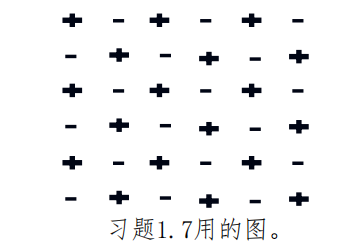
\includegraphics{picture/1-7.png} \end{center} ]{}
     
\proi{假设一固体中原子间的相互作用能可表示为:$U(r)=-\dfrac{\alpha}{r^m}+\dfrac{\beta}{r^n}$,试计算:\newline
        (1)平衡间距 ;\newline  
        (2)结合能W(单个原子的);\newline
        (3)体弹性模量;\newline
        (4)若取$m=2,n=10,r_0=0.3nm,W=0.4eV $,则$\alpha$和$\beta$的值是
        多少?}{}

\proi{设一固体平衡时体积为$V_0$, 原子间总的相互作用能为$U_0$, 如果原子间
    相互作用能由式$U(r)=-\dfrac{\alpha}{r^m}+\dfrac{\beta}{r^n}$所表述, 
    试证明体弹性模量为$\dfrac{nm|U_0|}{9V_0}$。}{}
     
\proi{对由N个正、负离子构成的离子固体, 假设其结合能为\[U(r)=\dfrac{N}{2}(-\dfrac{\alpha e^2}{4\pi \varepsilon_0 r}+\dfrac{\beta}{r^n})\]
    若以$ce^{-\dfrac{r}{\rho}}$来代替排斥项$\dfrac{\beta}{r_n}$, 当固体处于平衡时, 
    如果这两者对互作用势能的贡献相同, 试求$n$和$\rho$之间的关系。}{}
    
\proii{针对金刚石、石墨、碳60、碳纳米管和石墨烯五种碳同素异构体, 虽然它 
    们均是由纯碳原子构成的, 试分析为什么彼此间性能却有非常大的差别?}{}
        


\section{第二章}

\proi{试思考:最早的晶体是根据晶体具有鲜明宏观特征而发现的,但为什么说只 
    有恒定不变的晶面间夹角才是反映晶体的固有特征?恒定不变的晶面间夹角和晶体的微观结构特征有何关系?}
    {通过特征夹角的测定,可以判断所及晶体属于何种类型的晶体,而由其它宏观特征则不能。}

\proi{试思考:如何理解晶体、非晶体和准晶体?}
    {晶体既具有平移对称性又具有旋转对称性,准晶体只具有旋转对称性而不具有平移对称性,非晶体既不具有平移对称性又不具有旋转性。}

\proi{试思考:从晶格几何结构特征上,能否将金刚石结构和闪锌矿结构划归为同一类结构?}
    {不能。}
    
\proi{试思考:何谓布喇菲格子?布喇菲点阵中的格点如何进行表征?}
    {对由完全相同的一种原子周期性排布形成的单原子晶体,格点为原子平衡位置所在的几何点,这些格点在空间作周期性排布形成的格子称为布喇菲格子,也称简单格子。}

\proi{试思考:由同种原子形成的金刚石结构的晶体,如金刚石、硅等,如何理解 
        它们的晶格是复式格子而不是简单布喇菲格子? }
        {金刚石、硅等结构虽然由同种原子组成,但立方体顶角和面心原子同立方体体内原子的共价键取向不同,因此,金刚石、硅等结构的晶格属于复式格子而不是简单格子。}

\proi{试思考:如何理解空间点阵反映了晶体结构的几何特征?}
    {空间点阵是一种数学上的抽象,反映的是构成点阵的阵点在空间周期性排布 的几何特征,不具有任何实质性的物理内容。只有把基元放置于点阵的阵点位置上,才能形成具有特定晶体结构的晶体。可见,空间点阵和晶体结构,两者之间有密切的联系,但又是两个不同的概念,不能混淆。两者间的关系可概括为:点阵+基元=晶体结构。}

\proi{试思考:如何理解晶体的破缺平移对称性?}
    {通常所讲的空间平移对称性是指,若一个量具有空间平移对称性,则这个量不依赖于空间坐标原点的选择,将整个空间平移任意一个位置矢量,这个量的大小和性质保持不变。但对晶格来说,晶格并不对任意的空间平移保持不变,而只对从一个格点位置平移到另一格点位置才能保证晶格的不变性,因此,晶格的平移对称性是一种破缺的平移对称性。}

\proi{试思考: 如何理解晶体只有1,2,3,4和6的五个可能的旋转对称操作,而没有$n=5$以及$n>6$的旋转对称操作?}
    {尽管晶体的旋转操作是一种宏观操作,但要使得晶体在旋转操作后能自身重合,要求操作前后晶格点阵相同,而晶格是由格点的周期性排布而形成的,具有破缺的平移对称性,如下面的论证所看到的,这种破缺的平移对称性使得晶体不能在旋转任意角度下都能保证晶格点阵的不变,而只有在旋转为数不多的特定角度后晶格点阵才能保持不变,这和几何图形的正交变换大为不同。}

\proi{对于六角密堆积结构, 试证明:$\dfrac{c}{a}=(\dfrac{8}{3})^{\dfrac{1}{2}}$,如果明显大于此值, 则可能发生何种现象?}
    {如果$\dfrac{c}{a}=(\dfrac{8}{3})^{\dfrac{1}{2}}$,则相应的晶体为六角结构,但不是六角密积结构,在这种情况下,沿垂直于密面方向密排面之间呈现松散结合的特征。}
 
\proi{假定某种金属发生由体心立方结构到六角密堆积结构的结构相变, 若相变 时金属的密度维持不变且相变后六角密堆积结构相的$\dfrac{c}{a}$维持理想值, 试求相变后的晶格常数和相变前的晶格常数之间的关系。}
    {设相变前的晶格常数为$a_1$,相变后的晶格常数为$a_2、c_2$、;相变前后密度相同,\[ \dfrac{2}{a_1^3}=\dfrac{6}{3\sqrt{2}a_2^3}\]
        \[ \dfrac{a_2^3}{a_1^3}=\dfrac{1}{\sqrt{2}}\]}

\proi{将等体积的刚球分别排成简立方、体心立方、面心立方、六角密积和金刚石型的结构, 若以刚球体积与总体积之比表示晶体的致密度, 试针对不同的结构求晶体的致密度。}
    {简单立方:\[\rho=\dfrac{\pi}{6}\]
    体心立方:\[\rho=\dfrac{\pi \sqrt{3}}{8}\]
    面心立方:\[\rho=\dfrac{\pi \sqrt{2} }{6}\]
    六角密积:\[\rho=\dfrac{\pi \sqrt{2} }{6}\]
    金刚石型结构:\[\rho=\dfrac{\pi \sqrt{3} }{16}\]}

\proi{对体心立方和面心立方结构的晶体, 其固体物理学原胞的习惯选取如图 2. 23 所示, 试证明: 对体心立方晶体其原胞三基矢间的夹角为$109^o27'$, 对面心立方晶体其原胞三基矢间的夹角为$60^o$。}
    {体心立方晶体固体物理学原胞相对应的三个基矢以及相应原胞的体积分别为:\[\left\{\begin{array}{l}
     \vec{a}_{1}=\frac{a}{2}(-\vec{i}+\vec{j}+\vec{k}) \\
     \vec{a}_{2}=\frac{a}{2}(\vec{i}-\vec{j}+\vec{k}) \quad \text { 和 } \Omega=\vec{a}_{1} \bullet\left(\vec{a}_{2} \times \vec{a}_{3}\right)=\frac{1}{2} a^{3} \\
     \vec{a}_{3}=\frac{a}{2}(\vec{i}-\vec{j}+\vec{k}) 
    \end{array}\right.\]  \[\cos \theta=-\frac{1}{3}\] 面心立方结构晶体固体物理学原胞相对应的三个基矢和相应的原胞体积分别为:\[\left\{\begin{array}{l}
    \vec{a}_{1}=\frac{a}{2}(\vec{j}+\vec{k}) \\
    \vec{a}_{2}=\frac{a}{2}(\vec{i}+\vec{k}) \quad \text { 和 } \quad \Omega=\vec{a}_{1} \bullet\left(\vec{a}_{2} \times \vec{a}_{3}\right)=\frac{1}{4} a^{3}  \\
     \vec{a}_{3}=\frac{a}{2}(\vec{i}+\vec{j}) 
     \end{array}\right.\] \[ \cos \theta=\frac{1}{2}\]}

\proi{若某晶体的基矢为$\vec{a}_1=a\vec{i},\vec{a}_2=a\vec{j},\vec{a}_3=\frac{a}{2}(\vec{i}+\vec{j}+\vec{k})$, 试根据给定的基判断该晶体具有何种晶体结构?}
    {体心立方。}

\proi{试画出体心立方和面心立方晶格结构的晶体在(100),(110)和(111)晶面上的原子排列。}
    {略}

\proi{对如图所示的三维布喇菲格子,原胞的基矢方向如图所示,试求:\newline 
    (1)OA 晶列和 CA 晶列的晶向指数;\newline 
    (2)BCD 晶面和 ABC 晶面的面指数。}
    [\begin{center} 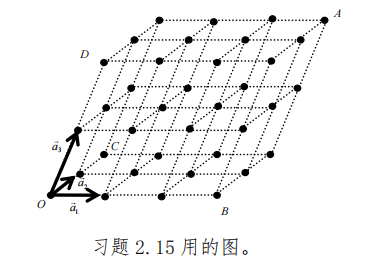
\includegraphics{picture/2-15.png} \end{center}]
    {(1)OA 晶列$[322]$  CA 晶列$[302]$\newline
    (2)BCD 晶面$(233)$ ABC 晶面$(32\bar{2})$}

\proi{ 考虑一个面心立方结构的晶体,其晶胞及基矢如图所示,A 是其中一个顶 
    角原子,B、C 是晶胞上的两个面心原子, 求:\newline(1)AC 晶列的晶向指数;\newline 
    (2)ABC 晶面的密勒指数。 }
    [\begin{center} 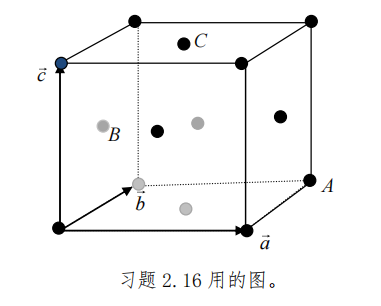
\includegraphics{picture/2-16.png} \end{center}]
    {(1)AC 晶列的晶向指数$[\bar{1}\bar{1}2]$\newline
    (2)ABC 晶面的密勒指数$(\bar{1}31)$}

\proii{已知三斜晶系的晶体中,三个基矢分别为$\vec{a}_1,\vec{a}_2 \text{和} \vec{a}_3$。现测知该晶体的 
    某一晶面法线与基矢的夹角依次为$\alpha,\beta \text{和} \gamma$,试求该晶面的面指数。}
    {\[(\dfrac{1}{|\vec{a}_1 \cos \alpha|},\dfrac{1}{|\vec{a}_2 \cos \beta|},\dfrac{1}{|\vec{a}_3 \cos \gamma|})\]}

\proii{对二维晶体,试论证二维平面点阵不可能有 5 度旋转对称轴。}
    {略}

\proii{石墨烯具有下图所示的正六角网状的结构形式,试问石墨烯的这种平面网 
    状格子是简单布喇菲格子还是复式格子?为什么?试画出固体物理学原胞和晶 
    胞。 }
    [ \begin{center} 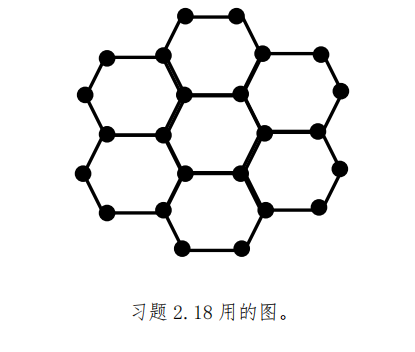
\includegraphics{picture/2-19-1.png}\end{center}]
    {石墨烯的这种平面网状格子是复式格子,若设石墨烯中相邻碳原子是等价的,会发现沿着A-B原子延伸出去1个单位的晶格平移矢量的地方其实并没有原子存在。也就说相邻的碳原子不等价,因为所处的环境并不相同。}
    [ \begin{center}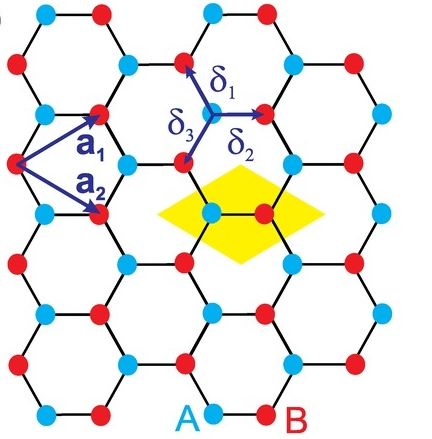
\includegraphics{picture/2-19-2.png} \end{center}]
        

\section{第三章}

\proi{试思考:从正格子空间到与之对应的傅里叶空间的变换,为什么不能采取通 
    常的坐标系变换的方式?}
    {晶体具有破缺的平移对称性,因此,对晶体而言,当从真实空间变换到与之对应的傅里叶空间时,其变换应不同于通常的傅里叶变换,或者说,在对晶体进行傅里叶变换时需要考虑晶体平移对称性破缺的事实。}

\proi{试思考:为什么说晶体中物理性质的平移对称性是破缺的? }
    {略。}

\proi{试思考:如何从正、倒格子不同角度来理解晶体结构的几何特征?}
    {略。}

\proi{试思考:如果$K_{h_1 h_2 h_3}=h_1\vec{b}_1+h_2\vec{b}_2+h_3\vec{b}_3$是任意的倒格矢,则该倒格矢的长度与晶面指数为$(h_1,h_2,h_3)$的晶面族面间距间的关系如何?}
    {\[\begin{gathered}
     d_{h_{1} h_{2} h_{3}}=\frac{\vec{a}_{1}}{h_{1}} \cdot \vec{e}_{n}=\frac{\vec{a}_{1}}{h_{1}} \cdot \frac{\vec{K}_{h_{1} h_{2} h_{3}}}{\left|\vec{K}_{h_{1} h_{2} h_{3}}\right|}=\frac{\vec{a}_{1}}{h_{1}} \cdot \frac{h_{1} \vec{b}_{1}+h_{2} \vec{b}_{2}+h_{3} \vec{b}_{3}}{\left|\vec{K}_{h_{1} h_{2} h_{3}}\right|} \\
     d_{h_{1} h_{2} h_{3}}=\frac{2 \pi}{\left|\vec{K}_{h_{1} h_{2} h_{3}}\right|}
    \end{gathered}\]}

\proi{试证明:简单六角布喇菲格子的倒格子仍为简单六角布喇菲格子,并给出其 
        倒格子空间的晶格常数。 }
        [\begin{center}
            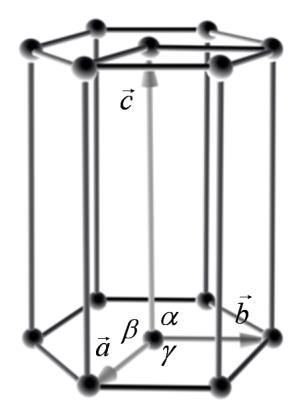
\includegraphics{picture/3-5.png}
        \end{center}]
       {六角晶系晶胞示意图, 其中$a=b\ne c ,\alpha=\beta=90^o$和$\gamma=120^o$
        利用下面公式:\[\left\{\begin{array}{l}
            \vec{b}_{1}=\frac{2 \pi}{\Omega}\left(\vec{a}_{2} \times \vec{a}_{3}\right) \\
            \vec{b}_{2}=\frac{2 \pi}{\Omega}\left(\vec{a}_{3} \times \vec{a}_{1}\right)  \\
            \vec{b}_{3}=\frac{2 \pi}{\Omega}\left(\vec{a}_{1} \times \vec{a}_{2}\right)
            \end{array}\right.\]可算得结果。(略)}

\proi{试证明:体心立方晶格的倒格子是具有面心立方结构的格子,而面心立方晶 
    格的倒格子是具有体心立方结构的格子。}
    {例如, 对晶格常数为  的体心立方格子, 根据固体物理学原胞的习惯选取方法,正格子空间的三个基矢在直角坐标系中分别表示为:$$
        \left\{\begin{array}{l}
        \overrightarrow{\mathrm{a}}_{1}=\frac{\mathrm{a}}{2}(-\overrightarrow{\mathrm{i}}+\overrightarrow{\mathrm{j}}+\overrightarrow{\mathrm{k}}) \\
        \overrightarrow{\mathrm{a}}_{2}=\frac{\mathrm{a}}{2}(\overrightarrow{\mathrm{i}}-\overrightarrow{\mathrm{j}}+\overrightarrow{\mathrm{k}}) \\
        \overrightarrow{\mathrm{a}}_{3}=\frac{\mathrm{a}}{2}(\overrightarrow{\mathrm{i}}+\overrightarrow{\mathrm{j}}-\overrightarrow{\mathrm{k}})
        \end{array}\right.
        $$
        原胞的体积 $\Omega=\overrightarrow{\mathrm{a}}_{1} \cdot\left(\overrightarrow{\mathrm{a}}_{2} \times \overrightarrow{\mathrm{a}}_{3}\right)=\frac{1}{2} \mathrm{a}^{3}$ 。代入到式 (3.8) 中可得到与体心立方正 格子相对应的倒格子空间的基矢为:
        $$
        \left\{\begin{array}{l}
        \vec{b}_{1}=\frac{2 \pi}{a}(\vec{j}+\vec{k}) \\
        \vec{b}_{2}=\frac{2 \pi}{a}(\vec{i}+\vec{k}) \\
        \vec{b}_{3}=\frac{2 \pi}{a}(\vec{i}+\vec{j})
        \end{array}\right.
        $$根据倒格子空间基矢的特征, 可以看到, 与体心立方正格子相对应的倒格子在倒格子空间中具有面心立方结构的格子特征。
        同理与面心立方正格子相对应的倒格子在倒格子空间中具有体心立方结构的格子特征(证明略)。}

\proi{试论证二维晶体的倒格子原胞面积和正格子原胞面积间的关系。 }
    {\[\left\{\begin{array}{l}
            \vec{b}_{1}=\frac{2 \pi}{|\vec{a}_{1} \times \vec{a}_{2}|}(\vec{a}_{2} \times \vec{e}_{3}) \\
            \vec{b}_{2}=\frac{2 \pi}{|\vec{a}_{1} \times \vec{a}_{2}|}(\vec{e}_{3} \times \vec{a}_{1})
            \end{array}\right.\]}
  
\proi{ 试证明正格子空间中一族晶面$(h_1h_2h_3)$和倒格矢$\vec{K}_{h}$正交。}
    {\[\vec{K}_{h_{1} h_{2} h_{3}} \cdot(\frac{\vec{a}_{1}}{h_{1}}-\frac{\vec{a}_{3}}{h_{3}})=0\]
        \[\vec{K}_{h_{1} h_{2} h_{3}} \cdot(\frac{\vec{a}_{2}}{h_{2}}-\frac{\vec{a}_{3}}{h_{3}})=0
        \]说明倒格矢$\vec{K}_{h}$与晶面$(h_1h_2h_3)$上的两个非平行的格矢正交。}

\proi{如果基矢$\vec{a},\vec{b},\vec{c}$构成简单正交系,试证明晶面族$(hkl)$的面间距为:$$
        d_{h k l}=\frac{1}{\sqrt{\left(\frac{h}{a}\right)^{2}+\left(\frac{k}{b}\right)^{2}+\left(\frac{l}{c}\right)^{2}}}
        $$并说明面指数简单的晶面, 其面密度比较大, 容易解理。}
        {简单正交杀 $\vec{a} \perp \vec{b} \perp \vec{c}$ $ \vec{a}_{1}=a\vec{i}, \vec{a}_{2}=b \vec{j}, \vec{a}_3=c\vec{k}$
        倒格子基矢 $\vec{b}_{1}=2 \pi \frac{\vec{a}_{2} \times \vec{a}_{3}}{\vec{a}_{1} \cdot (\vec{a}_{2} \times \vec{a}_{3})}, \quad \vec{b}_{2}=2 \pi \frac{\vec{a}_{3} \times \vec{a}_{1}}{\vec{a}_{1} \cdot(\vec{a}_{2} \times \vec{a}_{3})}, \quad \vec{b}_{3}=2 \pi \frac{\vec{a}_{1} \times \vec{a}_{2}}{\vec{a}_{1} \cdot (\vec{a}_{2} \times \vec{a}_{3})}$
        $$
        \vec{b}_{1}=\frac{2 \pi}{a} \vec{i}, \quad \vec{b}_{2}=\frac{2 \pi}{b} \vec{j}, \quad \vec{b}_{3}=\frac{2 \pi}{c} \vec{k}
        $$
        倒格子矢室 $\vec{G}=h \vec{b}_{1}+k \vec{b}_{2}+l \vec{b}_{3}=h \frac{2 \pi}{a} \vec{i}+k \frac{2 \pi}{b} \vec{j}+l \frac{2 \pi}{c} \vec{k}$ 晶面族  $(hkl)$ 的面间距
        $$
        d=\frac{2 \pi}{|\vec{G}|}=1 / \sqrt{(\frac{h}{a})^{2}+(\frac{k}{b})^{2}+(\frac{l}{c})^{2}}
        $$ 面指数越简单的晶面, 其晶面的间距越大,晶面上格点的密度越大, 这样的晶面越容易解理。}

\proi{对晶格常数为$a$的二维正方格子,试证明相应的倒格子仍然为正方格子并 
    给出倒格子空间的周期,试画出第一、第二和第三布里渊区。}
    {考虑边长为$a$的二维正方格子, 正格子空间的基矢为$\vec{a}_1=a\vec{i}$和$\vec{a}_2=a\vec{j}$。假设与之对应的倒格子空间的基矢为$\vec{b}_1=b_{11}\vec{i}+b_{12}\vec{j}$和$\vec{b}_2=b_{21}\vec{i}+b_{22}\vec{j}$, 利用正、倒格子基矢间的正交关系:$\vec{a}_i \cdot \vec{b}_j =2 \pi \delta_{ij}$, 则可得到$b_{11}=b_{22}=\dfrac{2 \pi}{a}$和$b_{12}=b_{21}=0$ , 因此, 与边长为$a$的二维正方格子相对应的倒格子的基矢为\[\vec{b}_1=\dfrac{2 \pi}{a}\vec{i} \text{和} \vec{b}_2=\dfrac{2 \pi}{a}\vec{j}\]
     可见, 与边长为  的二维正方格子相对应的倒格子仍为正方格子。}
     [\begin{center}
        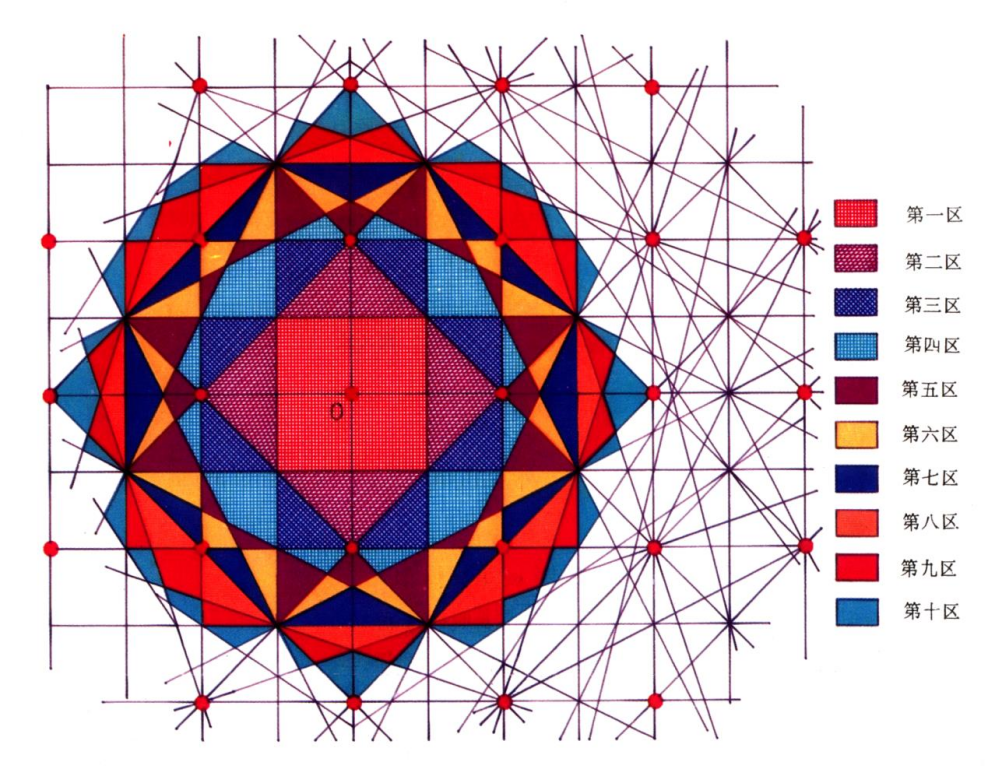
\includegraphics{picture/3-10 .png}
    \end{center}]

\proi{对晶格常数为$a$和$b$的二维矩形格子,试证明相应的倒格子仍然为二维矩形 
    格子并给出倒格子空间的周期,试画出第一布里渊区。}
    {同上题。(略)}

\proi{试问为什么面心立方晶体的第一布里渊区不是一个正八面体而是一个截角 
    的八面体?}
    [ \begin{center}
        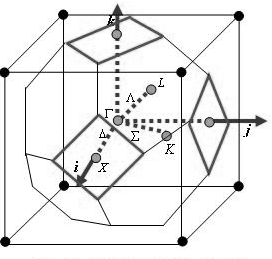
\includegraphics{picture/3-12.png}
    \end{center}]
    {对具有体心立方结构的倒格子, 每个倒格点同围有8个近邻倒格点。若选取立方体中心的倒格点作为原点$\Gamma$, 则在如图所示的直角坐标系中, 这8个近 邻倒格点的倒格矢分别为:
        \[\begin{aligned}
            &\frac{2 \pi}{a}(1,1,1), \frac{2 \pi}{a}(1,1, \overline{1}), \frac{2 \pi}{a}(1, \overline{1}, 1), \frac{2 \pi}{a}(\overline{1}, 1,1), \\
            &\frac{2 \pi}{a}(\overline{1}, \overline{1}, 1), \frac{2 \pi}{a}(\overline{1}, 1, \overline{1}), \frac{2 \pi}{a}(1, \overline{1}, \overline{1}), \frac{2 \pi}{a}(\overline{1}, \overline{1}, \overline{1}),
            \end{aligned}\]这 8 个倒格矢的中垂直面围成一个正八面体。稍加计算会发现, 这样一个正八面 体的体积会大于相应倒格子空间原胞的体积, 说明这样的正八面体不是面心立方 晶格的第一布里淋区。究其原因是, 原点$\Gamma$周围有六个次近邻倒格点, 这 6 个次近邻倒格点的倒格矢分别为:
            \[\frac{2 \pi}{a}(\pm 2,0,0), \frac{2 \pi}{a}(0, \pm 2,0), \frac{2 \pi}{a}(0,0, \pm 2)\]这六个倒格矢的中垂面截掉了正八面体的六个顶角, 形成如图  所示的裁角八面体, 变成了十四面体, 这样一个截角八面体(或者说十四面体)就是面心立方晶格的第一布里渊区。}


\section{第四章}

\proi{}{}

\proi{}{}

\proi{}{}


\section{第五章}

\proi{}{}

\proi{}{}

\proi{}{}


\section{第六章}

\proi{}{}

\proi{}{}

\proi{}{}


\section{第七章}

\proi{}{}

\proi{}{}

\proi{}{}



\end{document}
   